\section{Parallelized algorithms}
\label{sec:impl}

In the following implementations, we always use a similarity matrix with $1$ on its diagonal (symbols match) and $-1$ elsewhere (symbols do not match). The gap penalty is set to $p=-1$ (instead of $-2$ beforehand in the examples in \autoref{sec:needleman-wunsch}).

\subsection{On the CPU}

First, we implement the Needleman-Wunsch algorithm in Python using \tcboxverb{numpy}. This implementation serves well to deepen the understanding of the algorithm and to eliminate index errors. However, it is very slow, making it unsuitable for the whole dataset. We then translate the code to an unparallelized Rust version and confirm correct output by direct comparison with the Python implementation. To make use of all CPU cores, we \textbf{parallelize the Rust implementation} employing the \tcboxverb{rayon} library to parallelize the outer for-loop (\autoref{algstep:nested1}): for every word $A$, we consider all other words $B$ and calculate the similarity between $A$ and $B$. Since words lengths differ, the core calculation takes different times for different word pairs. Therefore, every thread appends its result to a vector that is wrapped in a \tcboxverb{Mutex} (avoid data races by mutual exclusion) and an \tcboxverb{Arc} (thread-safe reference pointer to deallocate data at the end).

Since comparing $A$ to $B$ yields the same score as the comparison of $B$ to $A$, we deal with \textit{undirected} edges and thus the adjacency matrix is symmetric. Furthermore, we are not interested in self-loops, but only in the similarity between \textit{different} words. For these two reasons, \textbf{we only consider the upper triangular part of the adjacency matrix} in \autoref{fig:traverse-schema}. To store the resulting edge weights in a binary file, we traverse the matrix in row-major order (red path): $(0,1)$, $(0,2)$, \ldots, $(0,n-1)$, $(1,2)$, \ldots, $(1,n-1), (2,3), \ldots, (n-2,n-1)$, where $n$ is the total number of words. Note that in the parallelized Rust implementation, we also have to the indices of the words since the order in which the threads terminate is not deterministic (from point of view of the Rust code). After all threads are finished, the results are sorted according to row-major ordering to match the traversal order. When saving the edge weights in a file, we drop the indices and only store the similarity scores as 8-bit signed integers (range $[-128,127]$). This is sufficient since word lengths are typically small and match/mismatch score as well as gap penalty $p$ are likewise chosen to be small.


\subsection{On the GPU}

We implement the algorithm in the CUDA framework and consult the \tcboxverb{cudarc} Rust library supplying Rust wrappers around the CUDA driver API as well as the NVRTC API (among others). The latter makes available methods to compile our \Cpp~kernel to \gls{ptx} code during runtime and to launch it.

\textbf{Subtasks.} Foster's PCAM methodology \cite{foster} can help in designing parallel algorithms. The first step is to partition the problem at hand into small tasks. At the level of the adjacency matrix (\autoref{fig:traverse-schema}), such a task would be to compute the similarity score between two words $A$ and $B$ at the respective row and column. On a finer granularity, we can also refer to \autoref{fig:matrix-nuance-puissance-subcalc} and consider the calculation of one element of the score matrix. However, we realize that latter calculations are highly dependent on each other since the score of a cell depends on the scores of its up, left and up-left (diagonal) neighbors (example of a \textit{stencil computation}). Additionally, words length differ, so the size of the score matrix varies. Due to the data dependencies and the varying problem size, we decide to focus on parallelizing the for-loops in the Needleman-Wunsch algorithm (lines \ref{algstep:nested1} and \ref{algstep:nested2} in \autoref{alg:needleman-wunsch}) making this a \textit{pleasingly parallel} problem, namely that of parallelizing score calculation for entries in the adjacency matrix.

\textbf{Grid.} The maximum number of blocks in a grid (grid size) is limited to $2^{16} - 1 = 65535$ in $y$ and $z$ direction. Starting with CUDA compute capability 3.0, the limit in the $x$ direction is raised to $2^{31} - 1 = 2,147,483,647$ blocks. Furthermore, we only consider the upper triangular part of the adjacency matrix, while a grid is always rectangular. These constraints motivate the choice of using a one-dimensional grid and spawning blocks only in the $x$ direction. Likewise, we only employ one-dimensional blocks, \ie a block is a one-dimensional array of threads. The exact number of threads we use inside a block (block dimension) is discussed later. With this configuration, we calculate (in every thread) an \textbf{index} ranging from $0$ to a number greater than that of entries in the upper triangular part of the adjacency matrix:
\begin{align}
    \text{idx} = \text{blockIdx.x} \cdot \text{blockDim.x} + \text{threadIdx.x}
    \label{eq:idx}
\end{align}
\textbf{Row \& Column}. The index \tcboxverb{idx} needs to be mapped to the corresponding row and column in the adjacency matrix, such that a thread knows which words to compare. We take advantage of the row-major traversal path. Let $S_r$ be the number of elements traversed up to the end of row $r$. In \autoref{fig:traverse-schema}, this variable is drawn in blue. \autoref{fig:sum-example} provides an example to ease keeping track during following calculations.

\begin{figure}[H]
    \centering
    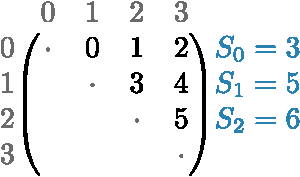
\includegraphics[width=0.5\linewidth]{assets/illustrator/sum-example.pdf}
    \caption{Example of \text{idx} (black) for $n=4$. $S_r$ is the number of elements traversed up to the end of row $r$ (blue).}
    \label{fig:sum-example}
\end{figure}

\vspace{-3em}

\begin{align}
    S_0 &= n-1, \quad S_1 = S_0 + (n-2), \quad\ldots\\
    S_r &= \sum_{k=0}^{r} (n-k-1)\\[-10pt]
    &= (n-1) \cdot (r+1) - \sum_{k=0}^{r} k\\[-2pt]
    &= (n-1) \cdot (r+1) - \frac{r \cdot (r+1)}{2}\\[-4pt]
    &= -\frac{1}{2}r^2 + r \left(n- \frac{3}{2}\right) + (n-1)
    \label{eq:sum-r}
\end{align}
For a given row $r$, we have $\text{idx} \in [S_{r-1}, S_r)$. Thus we require $S_{r-1} \overset{!}{=} \text{idx}$ and solve for $r$. After some algebraic manipulations, we obtain:
\begin{align}
    0 &= -\frac{1}{2} r^2 + r \underbrace{\left(n - \frac{1}{2}\right)}_z - \text{idx}\\
    \iff 0 &= r^2 + r (-2z) + 2 \cdot \text{idx}\\
    \implies r(\text{idx}) &= z - \sqrt{z^2 - 2\cdot \text{idx}}
    \label{eq:row-index}
\end{align}
We only use the negative branch of the square root since we want the row to \textit{increase} with increasing indices. Furthermore, we require the row index to be an integer, so we round down $\lfloor r(\text{idx}) \rfloor$, such that the row stays the same for a range of indices (those that refer to the same row). Column $c$ is then given by:
\begin{align}
    c(\text{idx}) &\coloneqq r + 1 + (\text{idx} - S_{r-1})\\
    &= \frac{1}{2} r^2 + r \left(\frac{3}{2} - n\right) + (\text{idx} + 1)
    \label{eq:col-index}
\end{align}
Finally, note that $S_{n-1}$ conveniently gives us the number of elements in the upper triangular part of the adjacency matrix, \ie the number of edges in our graph. With \eqref{eq:sum-r}, we find:
\begin{align}
    \small{\text{num edges}}
    &= S_{n-1} = \frac{1}{2} n^2 - \frac{1}{2} n
    = \frac{n(n-1)}{2}
    \label{eq:num-edges}
\end{align}

With \eqref{eq:row-index} and \eqref{eq:col-index}, we determine the respective row and column in the adjacency matrix for a given index \eqref{eq:idx}. During this row and column calculation, one should use 64-bit floating point numbers to mitigate precision errors that yield to wrong indices. Furthermore, we deal with graphs of more than $2^{32}$ edges and thus need to store the \tcboxverb{idx} as an 64-bit unsigned integer. The \tcboxverb{blockIdx.x} has to be statically cast to \tcboxverb{u64} (unsigned long long int), otherwise it is assumed to be \tcboxverb{u32} leading to incorrect indices and hard-to-debug errors for big graphs.

% \vspace{-0.3em}

\textbf{Memory.} In the first version of our CUDA kernel, for every thread we allocate an array of arrays on the heap inside global GPU memory for the score matrix.  We deallocate it after the alignment score is computed. This is very costly and immensely slows down the kernel execution. Instead, we want to use \textit{shared memory} for all threads in a block and let them share one big score matrix as to minimize the number of allocations needed. However, the score matrix dimensions differ in size depending on the word lengths of $A$ and $B$. Our solution is to look up the \underline{maximum word length $q$} before the kernel is launched, and allocate enough shared memory, \ie for every thread, we assume the worst-case scenario of a $(q+1)\times(q+1)$ matrix and allocate $(q+1)^2 \cdot \text{blockDim.x}$ chars (\tcboxverb{i8}) as linear shared memory. Then, inside each thread, we retrieve a pointer to the start of the memory reserved for this thread by adding $\text{threadIdx.x} \cdot (q+1)^2$ to the base pointer. To finally access element $(i,j)$ in the score matrix, we calculate $i\cdot \bigl(\lenn(B) + 1\bigr) + j$. This may not use all allocated memory, but it is a trade-off between memory usage and performance; with our approach we avoid bank conflicts.

% \vspace{-0.3em}

\textbf{Block dimension.} This dimension specifies the number of threads inside a block and is limited to 1024. We want to maximize shared memory available per block in order to minimize the number of memory allocations. Before the kernel is launched, for each $u\in [1,1024]$, the resulting shared memory size for one block ($u\cdot (q+1)^2$~bytes) is calculated. The greatest $u$ is chosen such that the maximum available shared memory per block (retrieved from CUDA device properties) is not exceeded.
